% !TeX program = xelatex

\documentclass[UTF8,a4paper,zihao=-4,fontset=windows]{ctexart}
% Shared renderer entrypoint for generated lessonplan.tex files.
% Generated documents should load ctexart, then input this file.

\usepackage{hepingjie_lessonplan}
% Hepingjie lesson-plan overlay coordinates.
% Coordinate origin: top-left corner of an A4 portrait page.
% Units: mm. These coordinates are frozen for templates/lessonplan/hepingjie_blank.pdf.

\newcommand{\LPBackgroundPdf}{templates/lessonplan/hepingjie_blank.pdf}

% Page 1 fixed fields.
\newcommand{\LPDateYearX}{65mm}
\newcommand{\LPDateMonthX}{89mm}
\newcommand{\LPDateDayX}{110mm}
\newcommand{\LPDateY}{38mm}
\newcommand{\LPRecordPageX}{170mm}
\newcommand{\LPRecordPageY}{38mm}

\newcommand{\LPTopicX}{32mm}
\newcommand{\LPTopicY}{49mm}
\newcommand{\LPTopicW}{108mm}
\newcommand{\LPTypeX}{154mm}
\newcommand{\LPTypeY}{49mm}
\newcommand{\LPTypeW}{40mm}

\newcommand{\LPUnitTotalX}{67mm}
\newcommand{\LPUnitTotalY}{61mm}
\newcommand{\LPTopicTotalX}{111mm}
\newcommand{\LPTopicTotalY}{61mm}
\newcommand{\LPCurrentPeriodX}{169mm}
\newcommand{\LPCurrentPeriodY}{61mm}

\newcommand{\LPBodyX}{33mm}
\newcommand{\LPObjectiveY}{74mm}
\newcommand{\LPObjectiveH}{39mm}
\newcommand{\LPKeyPointY}{119mm}
\newcommand{\LPKeyPointH}{15mm}
\newcommand{\LPDifficultyY}{137mm}
\newcommand{\LPDifficultyH}{15mm}
\newcommand{\LPMethodY}{156mm}
\newcommand{\LPMethodH}{15mm}
\newcommand{\LPMediaY}{174mm}
\newcommand{\LPMediaH}{15mm}
\newcommand{\LPBlackboardY}{196mm}
\newcommand{\LPBlackboardH}{73mm}
\newcommand{\LPBodyW}{164mm}

% Teaching process boxes on pages 2-4.
\newcommand{\LPProcessX}{33mm}
\newcommand{\LPProcessY}{31mm}
\newcommand{\LPProcessW}{163mm}
\newcommand{\LPProcessFullH}{249mm}
\newcommand{\LPProcessPageFourH}{160mm}


\usepackage{tikz}

\begin{document}

\LPBackgroundPage{1}{
  \LPCenterBox{\LPDateYearX}{\LPDateY}{12mm}{5mm}{}
  \LPCenterBox{\LPDateMonthX}{\LPDateY}{10mm}{5mm}{}
  \LPCenterBox{\LPDateDayX}{\LPDateY}{10mm}{5mm}{}
  \LPCenterBox{\LPRecordPageX}{\LPRecordPageY}{10mm}{5mm}{1}
  \LPTextBox{\LPTopicX}{\LPTopicY}{\LPTopicW}{8mm}{角的比较与运算}
  \LPTextBox{\LPTypeX}{\LPTypeY}{\LPTypeW}{8mm}{新授课}
  \LPCenterBox{\LPUnitTotalX}{\LPUnitTotalY}{12mm}{5mm}{7}
  \LPCenterBox{\LPTopicTotalX}{\LPTopicTotalY}{12mm}{5mm}{1}
  \LPCenterBox{\LPCurrentPeriodX}{\LPCurrentPeriodY}{12mm}{5mm}{1}
  \LPTextBox{\LPBodyX}{\LPObjectiveY}{\LPBodyW}{\LPObjectiveH}{\LPItems{\item 能用观察、叠合、度量比较角的大小。
\item 能根据图形写出角的和差关系并计算。
\item 能进行简单度分秒进位和借位运算。
\item 能应用角平分线进行基本求角。
}}
  \LPTextBox{\LPBodyX}{\LPKeyPointY}{\LPBodyW}{\LPKeyPointH}{角的比较方法、角的和差、度分秒运算和角平分线。}
  \LPTextBox{\LPBodyX}{\LPDifficultyY}{\LPBodyW}{\LPDifficultyH}{从图形中准确列式，并在度分秒减法中正确借位。}
  \LPTextBox{\LPBodyX}{\LPMethodY}{\LPBodyW}{\LPMethodH}{类比迁移; 动手测量; 图形观察; 板演计算; 纠错讨论}
  \LPTextBox{\LPBodyX}{\LPMediaY}{\LPBodyW}{\LPMediaH}{PPT; 黑板; 量角器; 三角板}
  \LPTextBox{\LPBodyX}{\LPBlackboardY}{\LPBodyW}{\LPBlackboardH}{\begin{enumerate}[leftmargin=1.4em,itemsep=0.4mm,topsep=0pt]
\item 比较：观察、叠合、度量。
\item 角大小只看张开程度，与边长无关。
\item 和差：$\angle AOC=\angle AOB+\angle BOC$。
\item 度分秒：$1^\circ=60'$，$1'=60''$。
\item 角平分线：从顶点出发，把角分成相等的两个角的射线。
\end{enumerate}}
}

\LPBackgroundPage{2}{
  \LPProcessBox{\LPProcessX}{\LPProcessY}{\LPProcessW}{\LPProcessFullH}{\LPProcessRow{导入与比较方法}{{\heiti 导入题}\par 问题1：两条边画得更长，角一定更大吗？学生可能误答“一定”。教师让学生看两个同样张开的角，指出角的大小看张开程度。问题2：线段可以相加、相减，角能否也用图形表示和差？引入本课。\par {\heiti 例题1 比较角的大小}\par 题目：比较图中两个角，左图边较长但张开较小，右图边较短但张开较大。\begin{center}\begin{tikzpicture}[scale=.62,baseline=(current bounding box.center)]\coordinate(O)at(0,0);\draw[->](O)--(3.2,0)node[right]{$A$};\draw[->](O)--(2.7,.55)node[right]{$B$};\node[left]at(O){$O$};\draw(.55,0)arc(0:11.5:.55);\node at(1.4,-.45){边较长，角较小};\begin{scope}[xshift=5.0cm]\coordinate(P)at(0,0);\draw[->](P)--(1.8,0)node[right]{$C$};\draw[->](P)--(.95,1.45)node[above]{$D$};\node[left]at(P){$P$};\draw(.48,0)arc(0:56:.48);\node at(1.15,-.45){边较短，角较大};\end{scope}\end{tikzpicture}\end{center}教师问：不用量角器怎样比较？规范方法：让顶点和一边重合，看另一边落在内部还是外部；也可用量角器度量。结论：角大小与边长无关。即时练习：判断“边越长角越大”是否正确，答：错误。备用题：画一个边短但角大的图，说明理由。}{\LPStudentItems{\item 观察两组角并先做直觉判断。
\item 用量角器验证判断。
\item 修正“边长决定角大小”的错误说法。
}}{10}
\LPProcessRow{角的和差关系}{{\heiti 例题2 角的和差关系}\par 题目：如图，射线 $OB$ 在 $\angle AOC$ 内部，写出角的和差关系。\begin{center}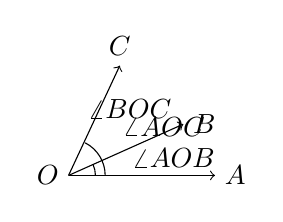
\begin{tikzpicture}[scale=.62]\coordinate(O)at(0,0);\coordinate(A)at(3,0);\coordinate(B)at(2.35,1.05);\coordinate(C)at(1.05,2.25);\draw[->](O)--(A)node[right]{$A$};\draw[->](O)--(B)node[right]{$B$};\draw[->](O)--(C)node[above]{$C$};\node[left]at(O){$O$};\draw(.55,0)arc(0:24:.55);\draw(.75,0)arc(0:63:.75);\node at(2.15,.35){$\angle AOB$};\node at(1.25,1.35){$\angle BOC$};\node at(1.95,1.0){$\angle AOC$};\end{tikzpicture}\end{center}关键问：大角由哪两个相邻小角组成？规范答：$\angle AOC=\angle AOB+\angle BOC$，$\angle BOC=\angle AOC-\angle AOB$。即时练习：若 $\angle AOC=80^\circ$，$\angle AOB=35^\circ$，则 $\angle BOC=45^\circ$。}{\LPStudentItems{\item 在图中标出 $A,O,B,C$。
\item 写出一个和式和两个差式。
\item 同桌检查角名顺序是否正确。
}}{8}}
}

\LPBackgroundPage{2}{
  \LPProcessBox{\LPProcessX}{\LPProcessY}{\LPProcessW}{\LPProcessFullH}{\LPProcessRow{度分秒运算}{{\heiti 例题3 度分秒运算}\par 题目：计算 $180^\circ-53^\circ17'$。教师问：0 分不够减 17 分怎么办？规范解：$180^\circ=179^\circ60'$，所以结果为 $126^\circ43'$。变式：$48^\circ35'+26^\circ40'=75^\circ15'$。即时练习：$90^\circ-37^\circ25'=52^\circ35'$。}{\LPStudentItems{\item 独立完成借位过程。
\item 说出 $179^\circ60'$ 的来源。
\item 把加法中满 60 分进 1 度。
}}{8}
\LPProcessRow{角平分线计算}{{\heiti 例题4 角平分线计算}\par 题目：$OB$ 平分 $\angle AOC$，且 $\angle AOC=76^\circ$，求 $\angle AOB$。\par\smallskip\noindent\begin{tikzpicture}[scale=.58]\coordinate(O)at(0,0);\coordinate(A)at(3,0);\coordinate(B)at(2.35,1.15);\coordinate(C)at(1.15,2.35);\draw[->](O)--(A)node[right]{$A$};\draw[->](O)--(B)node[right]{$B$};\draw[->](O)--(C)node[above]{$C$};\node[left]at(O){$O$};\draw(.55,0)arc(0:26:.55);\draw(.65,0)arc(0:26:.65);\draw(26:.55)arc(26:64:.55);\draw(26:.65)arc(26:64:.65);\node at(2.25,-.35){$OB$ 平分 $\angle AOC$};\end{tikzpicture}\par{}教师追问：相等的是哪两个角？规范解：$\angle AOB=\angle BOC=76^\circ\div2=38^\circ$。强调：角平分线是一条射线，必须从角的顶点出发。}{\LPStudentItems{\item 画出角平分线并标相等角。
\item 先求半角。
\item 说明角平分线是一条射线。
}}{4}
\LPProcessRow{综合计算}{{\heiti 例题5 综合计算}\par 题目：在上题基础上，若射线 $OD$ 在 $\angle BOC$ 内，且 $\angle COD=25^\circ$，求 $\angle BOD$。\par\smallskip\noindent\begin{tikzpicture}[scale=.54]\coordinate(O)at(0,0);\coordinate(A)at(3,0);\coordinate(B)at(2.35,1.1);\coordinate(D)at(1.75,1.75);\coordinate(C)at(.8,2.55);\draw[->](O)--(A)node[right]{$A$};\draw[->](O)--(B)node[right]{$B$};\draw[->](O)--(D)node[above right]{$D$};\draw[->](O)--(C)node[above]{$C$};\node[left]at(O){$O$};\draw(.5,0)arc(0:25:.5);\draw(.6,0)arc(0:25:.6);\draw(25:.5)arc(25:72:.5);\draw(25:.6)arc(25:72:.6);\draw(25:1.0)arc(25:45:1.0);\node at(2.35,.55){$B$在中间};\node at(1.55,1.55){$D$在$\angle BOC$内};\end{tikzpicture}\par{}规范解：先由角平分线得 $\angle BOC=38^\circ$，再看清 $OD$ 在 $\angle BOC$ 内，所以 $\angle BOD=38^\circ-25^\circ=13^\circ$。常见错误：没看清射线顺序，误用加法。}{\LPStudentItems{\item 按射线顺序读图。
\item 先求半角，再求相邻角之差。
\item 错题先补图再列式。
}}{3}}
}

\LPBackgroundPage{2}{
  \LPProcessBox{\LPProcessX}{\LPProcessY}{\LPProcessW}{\LPProcessFullH}{\LPProcessRow{必做练习与补救}{1. 若 $\angle AOC=96^\circ$，$OB$ 平分它，求 $\angle AOB$。2. 若 $\angle AOC=110^\circ$，$\angle AOB=37^\circ$，求 $\angle BOC$。3. 判断：角边越长角越大。答案：$48^\circ$；$73^\circ$；错误。巡视关注：角名顺序、半角计算和“边长决定角大小”的错误表述；正确率低时先重画射线顺序，再列和差式。}{\LPStudentItems{\item 独立完成三题。
\item 小组互查角名和单位。
\item 错题学生先画图，再补列式。
}}{7}
\LPProcessRow{看图提高与辨析}{提高题：如图，$OB$ 平分 $\angle AOC$，射线 $OD$ 在 $\angle BOC$ 内部，$\angle AOC=100^\circ$，$\angle BOD=18^\circ$，求 $\angle DOC$。\par\smallskip\noindent\begin{tikzpicture}[scale=.54]\coordinate(O)at(0,0);\coordinate(A)at(3,0);\coordinate(B)at(2.35,1.1);\coordinate(D)at(1.75,1.75);\coordinate(C)at(.8,2.55);\draw[->](O)--(A)node[right]{$A$};\draw[->](O)--(B)node[right]{$B$};\draw[->](O)--(D)node[above right]{$D$};\draw[->](O)--(C)node[above]{$C$};\node[left]at(O){$O$};\draw(.5,0)arc(0:25:.5);\draw(.6,0)arc(0:25:.6);\draw(25:.5)arc(25:72:.5);\draw(25:.6)arc(25:72:.6);\draw(25:1.0)arc(25:45:1.0);\node at(2.35,.55){$B$在中间};\node at(1.55,1.55){$D$在$\angle BOC$内};\end{tikzpicture}\par{}解：$\angle BOC=100^\circ\div2=50^\circ$，$\angle DOC=50^\circ-18^\circ=32^\circ$。图形辨析题：\par\smallskip\noindent\begin{tikzpicture}[scale=.46]\coordinate(O)at(0,0);\draw[->](O)--(2.6,0)node[right]{$A$};\draw[->](O)--(2.05,1.0)node[right]{$B$};\draw[->](O)--(1.0,2.2)node[above]{$C$};\node[left]at(O){$O$};\draw(.45,0)arc(0:26:.45);\draw(.55,0)arc(0:26:.55);\draw(26:.45)arc(26:66:.45);\draw(26:.55)arc(26:66:.55);\node at(1.25,-.4){图1 有相等标记};\begin{scope}[xshift=6.1cm]\coordinate(P)at(0,0);\draw[->](P)--(2.6,0)node[right]{$A$};\draw[->](P)--(1.9,.75)node[right]{$B$};\draw[->](P)--(1.0,2.2)node[above]{$C$};\node[left]at(P){$O$};\draw(.5,0)arc(0:65:.5);\node at(1.25,-.4){图2 只有内部射线};\end{scope}\end{tikzpicture}\par{}能否仅根据 $OB$ 在角内部判断它是角平分线？答：不能，必须有已知条件或相等角标记。两题均为备用/机动题，不另计固定时间。}{\LPStudentItems{\item 完成较快者做机动题。
\item 指出图中已知标记。
\item 不能只凭视觉说平分。
}}{0}
\LPProcessRow{反馈测试与小结}{{\heiti 课堂反馈测试 5分}\par 共 10 分。1. 角的大小与边长有关吗？2分。2. 若 $OB$ 在 $\angle AOC$ 内部，写一个和式和一个差式。2分。3. 计算 $70^\circ-28^\circ45'$，3分。4. $OD$ 平分 $\angle AOB$，$\angle AOB=64^\circ$，求 $\angle AOD$，3分。答案：无关；$\angle AOC=\angle AOB+\angle BOC$；$41^\circ15'$；$32^\circ$。学生自评，教师抽查度分借位错例。}{\LPStudentItems{\item 完成反馈测试并自评。
\item 说出本节一个方法、一个公式和一个易错点。
\item 用错例说明角名和单位不能混。
}}{5}}
}

\LPBackgroundPage{4}{
  \LPProcessBox{\LPProcessX}{\LPProcessY}{\LPProcessW}{\LPProcessPageFourH}{\LPProcessRow{分层作业}{A组：1. 说明角大小由什么决定。2. 画图表示 $\angle AOC=\angle AOB+\angle BOC$。3. 计算 $63^\circ20'+18^\circ50'$。4. 计算 $120^\circ-46^\circ35'$。5. 若角平分线把 $86^\circ$ 分成两角，求每个角。B组：1. 已知 $\angle AOC=105^\circ$，$\angle BOC=39^\circ$，求 $\angle AOB$。2. 判断“角平分线是角内部一个点”并改正。3. 画三条射线并写两个角的和差式。C组选做：设计一道含角平分线和度分秒减法的题并给答案。答案：A3 $82^\circ10'$，A4 $73^\circ25'$，A5 $43^\circ$，B1 $66^\circ$。}{\LPStudentItems{\item 记录分层作业。
\item A组全员完成，B组选做订正，C组学有余力完成。
\item 选做题可课后交流。
}}{0}}
}

\end{document}
